\begin{figure}[h!]
	\begin{subfigure}{\linewidth}
		\caption{}
		\centering
		% include first image
		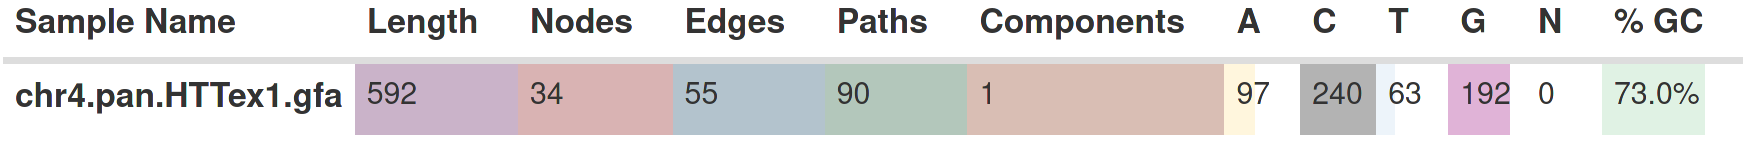
\includegraphics[width=1.0\linewidth, trim=-1.25cm 3cm 0 1.75cm]{fig/metrics/chr4_pan_HTTex1_gfa_multiqc_odgi_stats}
		\label{fig:metrics-multiqc}
	\end{subfigure}
	\begin{subfigure}{1\linewidth}
	\caption{}
	\centering
	% include fourth image
	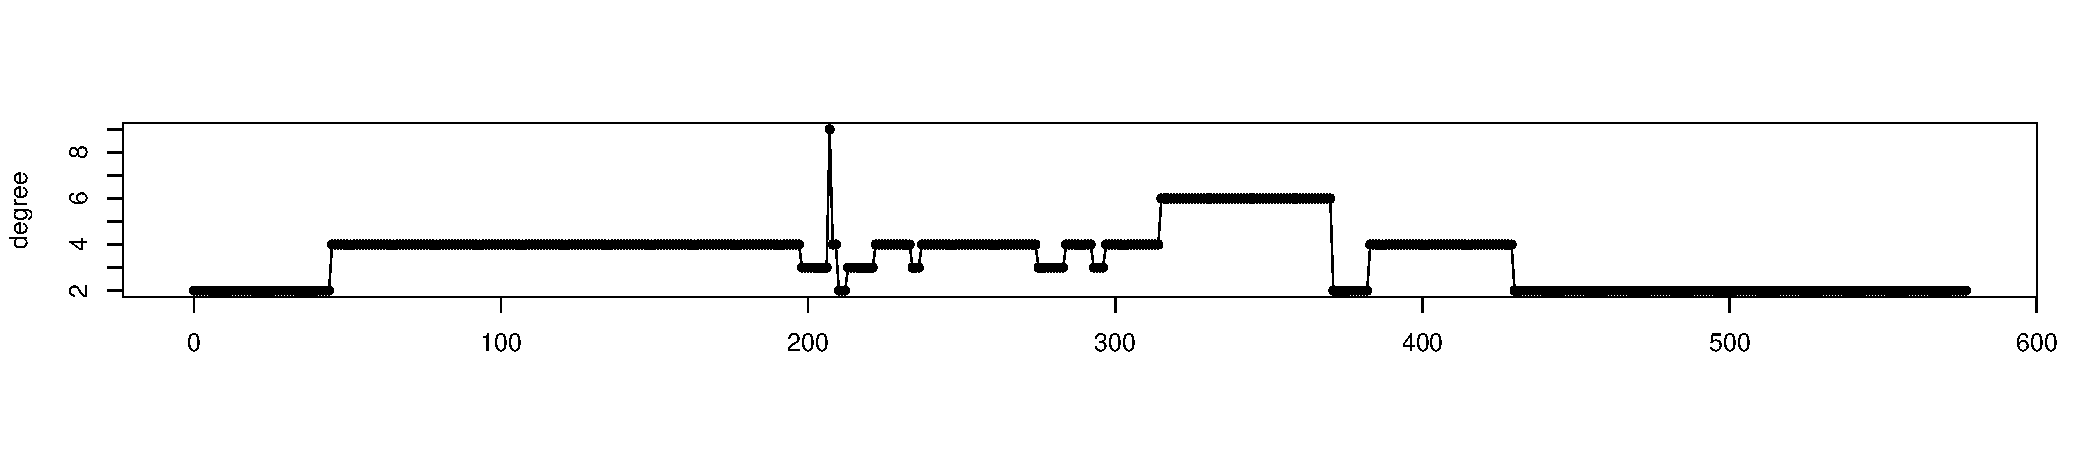
\includegraphics[width=\linewidth,trim=+.225cm 3cm +.425cm +3cm]{fig/metrics/chr4_HTT_chm13_degree_w1_bed}
	\label{fig:metrics-degree}
	\end{subfigure}
	\begin{subfigure}{\linewidth}
	\caption{}
	\centering
	% include second image
	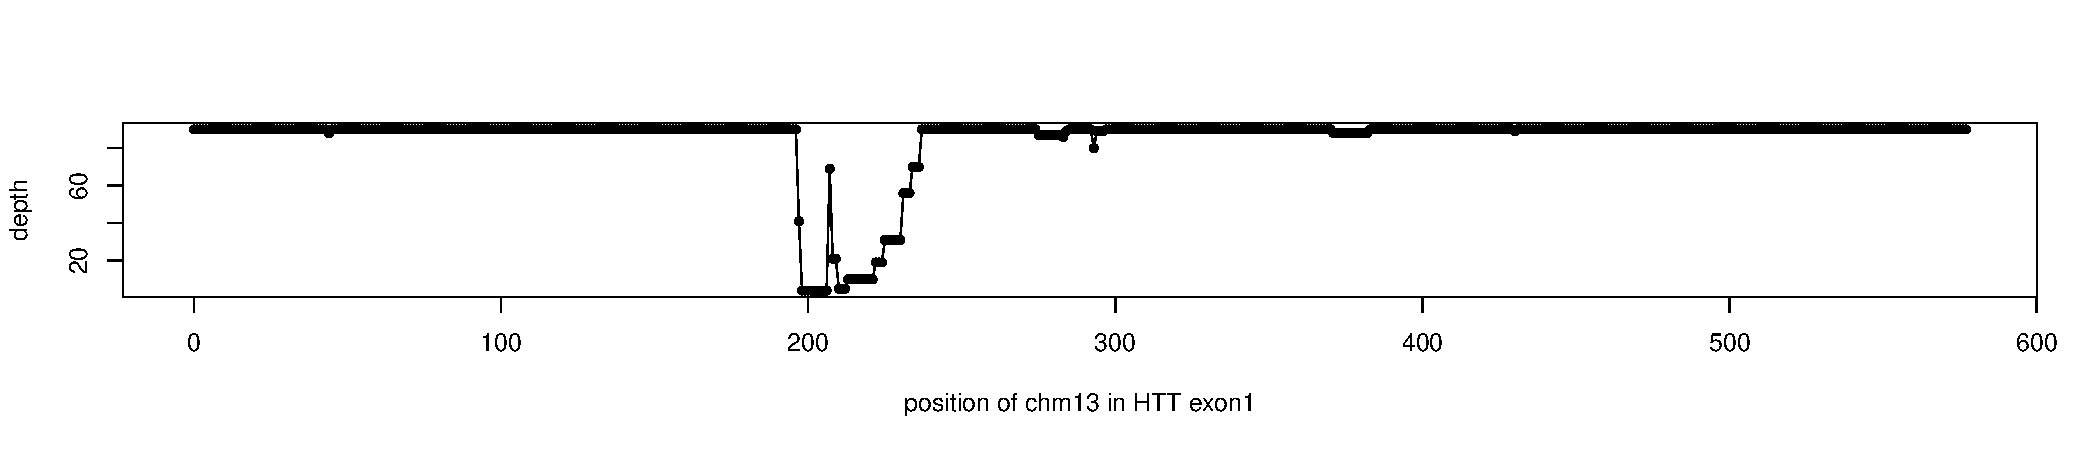
\includegraphics[width=\linewidth,trim=+.225cm 3cm +0.425cm +3cm]{fig/metrics/chr4_HTT_chm13_depth_w1_bed}
	\label{fig:metrics-depth}
	\end{subfigure}
	\begin{subfigure}{\linewidth}
		\caption{}
		\centering
		% include second image
		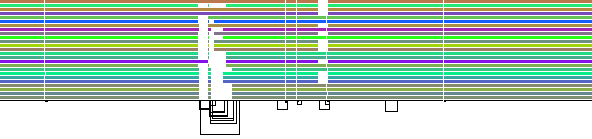
\includegraphics[width=1.0\linewidth, trim=-1.95cm 2cm -1.0cm 0.5cm]{fig/metrics/chr4_pan_fa_a2fb268_e820cd3_9ea71d8_smooth_gfa_og_HTTex1_og_O_og_tiny_og}
		\label{fig:metrics-viz}
	\end{subfigure}
%	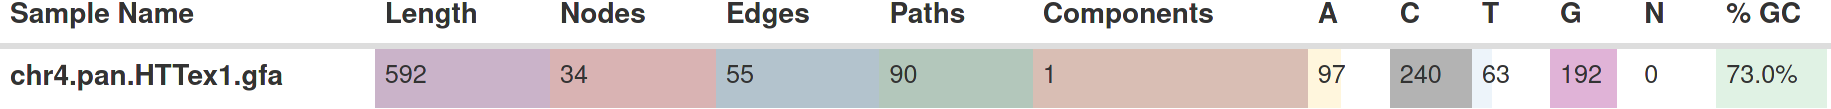
\includegraphics[width=\linewidth]{fig/metrics/chr4.pan.HTTex1.gfa.multiqc_odgi_stats.png}
	\caption{Features of a 90 haplotypes human pangenome graph of the exon 1 huntingtin gene (\textit{HTTexon1}): \textbf{(a)} Excerpt of vital statistics of the \textit{HTTexon1} graph displayed by MultiQC's ODGI module. The very high GC content of 73.0\% compared to a human genomic mean GC content of 40.9\% \cite{Piovesan2019} is in accordance with the literature (see for example \cite{Sathasivam2013, Neueder2017}). \textbf{(b)} Per nucleotide node degree distribution of CHM13 in the \textit{HTTexon1} graph. Around position 200 there is a huge variation in node degree. \textbf{(c)} Per nucleotide node depth distribution of CHM13 in the \textit{HTTexon1} graph. The alternating depth around position 200 indicates polymorphic variation complementing the above node degree analysis. \textbf{(d)} \textit{odgi viz} visualization of the 23 largest gene alleles, CHM13, and GRCH38 of the \textit{HTTexon1} graph. Figures \textbf{(b)-(d)} clearly highlight the variant region around position 200 showing the variable number of glutamine residues of the different individuals as reported by \cite{Nance1999}.}
	\label{fig:metrics}
\end{figure}
